\chapter{Les lois de Newton}

\textit{La mécanique newtonienne constitue le socle de la physique classique. Ce chapitre établit les trois lois fondamentales qui régissent le mouvement des corps, en introduisant les outils vectoriels nécessaires à leur description : position, vitesse, accélération et quantité de mouvement. Ces lois permettent de relier les causes (forces) aux effets (mouvements) et ouvrent la voie à l’étude de systèmes aussi variés qu’un projectile, un satellite ou un véhicule en mouvement.}

% ============================================================
\section{Rappels cinématiques : vecteurs position, vitesse et accélération}

\begin{definition}[Vecteur position]
Dans un référentiel muni d’un repère orthonormé $(O,\vect{i},\vect{j},\vect{k})$, le vecteur position d’un point $M$ à l’instant $t$ est :
\[
\vect{OM}(t) = x(t)\,\vect{i} + y(t)\,\vect{j} + z(t)\,\vect{k}.
\]
\end{definition}

\begin{definition}[Vecteur vitesse]
Le vecteur vitesse instantanée est la dérivée par rapport au temps du vecteur position :
\[
\vect{v}(t) = \dv{\vect{OM}}{t} = \dot{x}(t)\,\vect{i} + \dot{y}(t)\,\vect{j} + \dot{z}(t)\,\vect{k}.
\]
Sa norme $v = \|\vect{v}\|$ s’exprime en \si{\metre\per\second}.
\end{definition}

\begin{definition}[Vecteur accélération]
Le vecteur accélération instantanée est la dérivée du vecteur vitesse :
\[
\vect{a}(t) = \dv{\vect{v}}{t} = \ddot{x}(t)\,\vect{i} + \ddot{y}(t)\,\vect{j} + \ddot{z}(t)\,\vect{k}.
\]
Unité : \si{\metre\per\second\squared}.
\end{definition}

\begin{remarque}
En coordonnées cartésiennes, les composantes de $\vect{v}$ et $\vect{a}$ s’obtiennent par simple dérivation des fonctions $x(t)$, $y(t)$, $z(t)$.
\end{remarque}

\subsection{Repère de Frenet}

Pour un mouvement curviligne, on utilise le repère de Frenet $(\vect{T},\vect{N})$ où $\vect{T}$ est le vecteur unitaire tangent à la trajectoire et $\vect{N}$ le vecteur unitaire normal dirigé vers le centre de courbure.

\begin{propriete}[Expressions dans le repère de Frenet]
\[
\vect{v} = v\,\vect{T}, \qquad
\vect{a} = \dv{v}{t}\,\vect{T} + \frac{v^{2}}{R}\,\vect{N},
\]
où $R$ est le rayon de courbure local de la trajectoire.
\end{propriete}

\begin{illus}
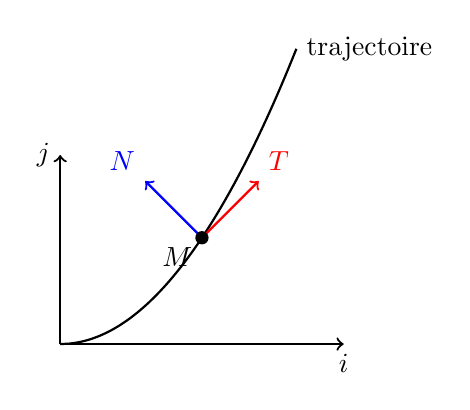
\begin{tikzpicture}[scale=1.2]
\draw[thick,->] (0,0) -- (3,0) node[below]{$\vect{i}$};
\draw[thick,->] (0,0) -- (0,2) node[left]{$\vect{j}$};
\draw[domain=0:2.5,smooth,variable=\x,thick] plot ({\x},{0.5*\x*\x}) node[right]{trajectoire};
\draw[->,red,thick] (1.5,1.125) -- ++(0.6,0.6) node[above right]{$\vect{T}$};
\draw[->,blue,thick] (1.5,1.125) -- ++(-0.6,0.6) node[above left]{$\vect{N}$};
\fill (1.5,1.125) circle (2pt) node[below left]{$M$};
\end{tikzpicture}
\fig{Figure 2.1 — Repère de Frenet le long d’une trajectoire parabolique.}
\end{illus}

% ============================================================
\section{Référentiels galiléens et quantité de mouvement}

\begin{definition}[Référentiel galiléen]
Un référentiel est dit galiléen si le principe d’inertie (1\iere{} loi de Newton) y est vérifié : tout point matériel isolé (ou pseudo-isolé) y persévère dans son état de repos ou de mouvement rectiligne uniforme.
\end{definition}

\begin{exemple}
Le référentiel terrestre est considéré galiléen pour des expériences de courte durée devant la rotation de la Terre. Le référentiel héliocentrique est galiléen pour l’étude du mouvement des planètes.
\end{exemple}

\begin{definition}[Quantité de mouvement]
Pour un point matériel de masse $m$ et de vitesse $\vect{v}$, la quantité de mouvement est :
\[
\vect{p} = m\,\vect{v}.
\]
Unité : \si{\kilogram\metre\per\second}.
\end{definition}

\begin{remarque}
La quantité de mouvement est une grandeur vectorielle additive pour un système de points.
\end{remarque}

% ============================================================
\section{Les trois lois de Newton}

\subsection{Première loi : principe d’inertie}

\begin{loi}[Principe d’inertie]
Dans un référentiel galiléen, un point matériel soumis à un ensemble de forces dont la résultante est nulle ($\sum \vect{F} = \vect{0}$) conserve sa quantité de mouvement : $\vect{p} = \text{constante}$. En particulier, si $\vect{v}_0 = \vect{0}$, le corps reste au repos.
\end{loi}

\begin{aretenir}
Le principe d’inertie définit les référentiels galiléens et établit l’équivalence entre repos et mouvement rectiligne uniforme en l’absence de force résultante.
\end{aretenir}

\subsection{Deuxième loi : relation fondamentale de la dynamique}

\begin{loi}[Relation fondamentale de la dynamique]
Dans un référentiel galiléen, la dérivée par rapport au temps de la quantité de mouvement d’un point matériel est égale à la somme des forces qui lui sont appliquées :
\[
\dv{\vect{p}}{t} = \sum \vect{F}.
\]
Si la masse est constante, on obtient la forme usuelle :
\[
m\,\vect{a} = \sum \vect{F}.
\]
\end{loi}

\begin{exemple}
Pour une chute libre sans frottement, la seule force est le poids $\vect{P}=m\vect{g}$. La 2\ieme{} loi donne $m\vect{a}=m\vect{g}$, soit $\vect{a}=\vect{g}$ : le mouvement est uniformément accéléré.
\end{exemple}

\subsection{Troisième loi : principe des actions réciproques}

\begin{loi}[Principe des actions réciproques]
Lorsque deux corps $A$ et $B$ sont en interaction, la force exercée par $A$ sur $B$ est opposée à celle exercée par $B$ sur $A$ :
\[
\vect{F}_{A\to B} = -\vect{F}_{B\to A}.
\]
Ces forces sont de même direction, de même intensité mais de sens contraire.
\end{loi}

\begin{remarque}
Les deux forces s’appliquent sur des corps différents : elles ne se compensent pas.
\end{remarque}

% ============================================================
\section{Bilan des forces et théorème du centre d’inertie}

\subsection{Méthode du bilan des forces}

Pour appliquer la 2\ieme{} loi, il faut recenser toutes les forces extérieures agissant sur le système étudié. Les forces usuelles sont :
\begin{itemize}
\item le poids $\vect{P}=m\vect{g}$ (vertical, vers le bas) ;
\item la réaction normale $\vect{R}_N$ (perpendiculaire au support) ;
\item la force de frottement $\vect{f}$ (tangentielle, opposée au mouvement) ;
\item la tension d’un fil $\vect{T}$ (dirigée le long du fil) ;
\item la poussée d’Archimède $\vect{\Pi}$ (verticale, vers le haut).
\end{itemize}

\begin{illus}
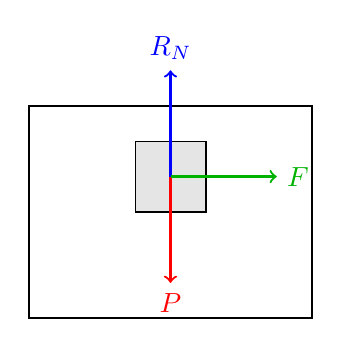
\begin{tikzpicture}[scale=0.9]
\draw[thick] (0,0) -- (4,0) -- (4,3) -- (0,3) -- cycle;
\draw[fill=gray!20] (1.5,1.5) rectangle (2.5,2.5);
\draw[->,red,thick] (2,2) -- (2,0.5) node[below]{$\vect{P}$};
\draw[->,blue,thick] (2,2) -- (2,3.5) node[above]{$\vect{R}_N$};
\draw[->,green!70!black,thick] (2,2) -- (3.5,2) node[right]{$\vect{F}$};
\end{tikzpicture}
\fig{Figure 2.2 — Bilan des forces sur un bloc posé sur un plan horizontal : poids, réaction normale, force de traction.}
\end{illus}

\subsection{Théorème du centre d’inertie}

\begin{propriete}[Théorème du centre d’inertie]
Pour un système de points matériels de masse totale $M$, le centre d’inertie $G$ se comporte comme un point matériel de masse $M$ soumis à la résultante des forces extérieures $\vect{F}_{\text{ext}}$ :
\[
M\,\vect{a}_G = \sum \vect{F}_{\text{ext}}.
\]
\end{propriete}

\begin{remarque}
Ce théorème permet d’étudier le mouvement global d’un système sans détailler les forces intérieures.
\end{remarque}

% ============================================================
\section{Application au plan incliné}

\begin{experience}[Mouvement sur un plan incliné]
Un solide de masse $m$ glisse sans frottement sur un plan incliné d’un angle $\alpha$ par rapport à l’horizontale. Le bilan des forces donne le poids $\vect{P}$ et la réaction normale $\vect{R}_N$. En projetant sur l’axe parallèle au plan, on obtient :
\[
m a = m g \sin\alpha \quad\Rightarrow\quad a = g \sin\alpha.
\]
\end{experience}

\begin{illus}
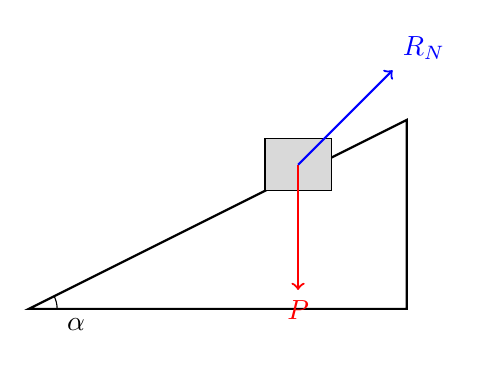
\begin{tikzpicture}[scale=1.2]
\draw[thick] (0,0) -- (4,0) -- (4,2) -- cycle;
\draw[fill=gray!30] (2.5,1.25) rectangle (3.2,1.8);
\draw[->,red,thick] (2.85,1.525) -- (2.85,0.2) node[below]{$\vect{P}$};
\draw[->,blue,thick] (2.85,1.525) -- (3.85,2.525) node[above right]{$\vect{R}_N$};
\draw (0,0) -- (0.5,0) node[below]{$\alpha$};
\draw (0.3,0) arc (0:26.565:0.3);
\end{tikzpicture}
\fig{Figure 2.3 — Solide sur un plan incliné : décomposition du poids.}
\end{illus}

% ============================================================
\section{L’essentiel à retenir}

\begin{synthese}
\begin{itemize}
\item \textbf{Vecteurs cinématiques :} $\vect{v}=\dv{\vect{OM}}{t}$, $\vect{a}=\dv{\vect{v}}{t}$.
\item \textbf{Repère de Frenet :} $\vect{v}=v\vect{T}$, $\vect{a}=\dot{v}\vect{T}+\dfrac{v^{2}}{R}\vect{N}$.
\item \textbf{Quantité de mouvement :} $\vect{p}=m\vect{v}$.
\item \textbf{1\iere{} loi :} $\sum\vect{F}=\vect{0}\;\Leftrightarrow\;\vect{p}=\text{cte}$ (référentiel galiléen).
\item \textbf{2\ieme{} loi :} $\dv{\vect{p}}{t}=\sum\vect{F}$ ou $m\vect{a}=\sum\vect{F}$ (masse constante).
\item \textbf{3\ieme{} loi :} $\vect{F}_{A\to B}=-\vect{F}_{B\to A}$.
\item \textbf{Théorème du centre d’inertie :} $M\vect{a}_G=\sum\vect{F}_{\text{ext}}$.
\item \textbf{Unités :} $v$ en \si{\metre\per\second}, $a$ en \si{\metre\per\second\squared}, $p$ en \si{\kilogram\metre\per\second}, $F$ en \si{\newton}.
\item \textbf{Piège :} Ne pas oublier que les forces intérieures ne modifient pas le mouvement du centre d’inertie.
\end{itemize}
\end{synthese}

% ============================================================
\section{Méthodes \& savoir-faire}

\methode{Appliquer la relation fondamentale de la dynamique}
\begin{enumerate}
\item Définir le système et le référentiel galiléen.
\item Faire le bilan des forces extérieures.
\item Choisir un repère adapté (cartésien ou de Frenet).
\item Écrire $m\vect{a}=\sum\vect{F}$ et projeter sur les axes.
\item Résoudre les équations différentielles obtenues.
\end{enumerate}
\begin{exemple}
Un parachutiste de masse $m=\SI{80}{\kilogram}$ est soumis à son poids et à une force de frottement fluide $\vect{f}=-k\vect{v}$ ($k=\SI{15}{\newton\second\per\metre}$). En projetant sur l’axe vertical descendant, on a $m\dot{v}=mg-kv$. La solution donne $v(t)=\frac{mg}{k}(1-e^{-kt/m})$.
\end{exemple}

\methode{Utiliser le repère de Frenet}
Pour un mouvement circulaire uniforme de rayon $R$, $\dot{v}=0$ donc $\vect{a}=\frac{v^{2}}{R}\vect{N}$. La 2\ieme{} loi donne la force centripète nécessaire.
\begin{exemple}
Une voiture de masse $m=\SI{1200}{\kilogram}$ prend un virage de rayon $R=\SI{50}{\metre}$ à $v=\SI{72}{\kilo\metre\per\hour}$. La force de frottement latérale vaut $f=m v^{2}/R=\SI{9600}{\newton}$.
\end{exemple}

\methode{Appliquer le principe des actions réciproques}
Lors de l’étude d’un système de deux corps en interaction, on écrit $\vect{F}_{1\to2}=-\vect{F}_{2\to1}$ et on applique la 2\ieme{} loi à chaque corps séparément.
\begin{exemple}
Deux patineurs de masses $m_1=\SI{60}{\kilogram}$ et $m_2=\SI{80}{\kilogram}$ se repoussent. Si $m_1$ acquiert une accélération $a_1=\SI{2}{\metre\per\second\squared}$, alors $a_2=-m_1 a_1/m_2=\SI{-1.5}{\metre\per\second\squared}$.
\end{exemple}

\methode{Étudier un mouvement sur un plan incliné}
\begin{enumerate}
\item Orienter l’axe $x$ parallèlement au plan (sens de la descente) et $y$ perpendiculaire.
\item Projeter le poids : $P_x=mg\sin\alpha$, $P_y=-mg\cos\alpha$.
\item Écrire $ma_x=mg\sin\alpha$ (sans frottement) et $a_y=0$ (pas de décollement).
\end{enumerate}
\begin{exemple}
Un skieur de $m=\SI{70}{\kilogram}$ descend une pente à $\alpha=\ang{30}$ sans frottement. Son accélération est $a=g\sin\ang{30}=\SI{4.9}{\metre\per\second\squared}$.
\end{exemple}

\methode{Appliquer le théorème du centre d’inertie}
Pour un système de plusieurs points, on calcule la position de $G$ par $\vect{OG}=\frac{1}{M}\sum m_i\vect{OM}_i$, puis on applique $M\vect{a}_G=\sum\vect{F}_{\text{ext}}$.
\begin{exemple}
Deux masses $m_1=\SI{2}{\kilogram}$ et $m_2=\SI{3}{\kilogram}$ reliées par un fil sont tirées par une force $\vect{F}=\SI{10}{\newton}$ horizontale. L’accélération du centre d’inertie est $a_G=F/(m_1+m_2)=\SI{2}{\metre\per\second\squared}$.
\end{exemple}

\methode{Passer des lois de Newton aux équations horaires}
Après avoir obtenu $\vect{a}$, on intègre pour trouver $\vect{v}(t)$ puis $\vect{OM}(t)$ en tenant compte des conditions initiales.
\begin{exemple}
Pour une chute libre avec $v_0$ verticale vers le bas, $a=g$, $v(t)=v_0+gt$, $z(t)=z_0+v_0 t+\frac{1}{2}gt^{2}$.
\end{exemple}

% ============================================================
\section{Exercices d’application}

\rubrique{Cinématique vectorielle}

\exo{}\diff{1} Un mobile se déplace selon $x(t)=3t^{2}-2t+1$ (en mètres). Déterminer les expressions de $v_x(t)$ et $a_x(t)$. Calculer $v_x$ à $t=\SI{2}{\second}$.

\exo{}\diff{2} Un point $M$ décrit une trajectoire circulaire de rayon $R=\SI{0.5}{\metre}$ à vitesse constante $v=\SI{2}{\metre\per\second}$. Calculer son accélération normale.

\rubrique{Quantité de mouvement et 2\ieme{} loi}

\exo{}\diff{1} Une balle de masse $m=\SI{50}{\gram}$ est lancée à $v=\SI{20}{\metre\per\second}$. Quelle est sa quantité de mouvement ?

\exo{}\diff{2} Une voiture de masse $m=\SI{1000}{\kilogram}$ passe de $0$ à $\SI{90}{\kilo\metre\per\hour}$ en $\SI{10}{\second}$. Calculer la force moyenne exercée par le moteur (on néglige les frottements).

\rubrique{Bilan des forces et plan incliné}

\exo{}\diff{2} Un bloc de masse $m=\SI{5}{\kilogram}$ glisse sans frottement sur un plan incliné de $\alpha=\ang{20}$. Déterminer son accélération et la réaction normale.

\exo{}\diff{3} Reprendre l’exercice précédent avec un coefficient de frottement $\mu=0.15$. Calculer la nouvelle accélération.

\rubrique{Principe des actions réciproques}

\exo{}\diff{2} Deux chariots de masses $m_1=\SI{2}{\kilogram}$ et $m_2=\SI{3}{\kilogram}$ sont reliés par un ressort. On les écarte puis on les lâche. Si $m_1$ a une accélération $a_1=\SI{1.5}{\metre\per\second\squared}$, quelle est l’accélération de $m_2$ ?

\rubrique{Théorème du centre d’inertie}

\exo{}\diff{2} Un système de trois masses $m_1=\SI{1}{\kilogram}$, $m_2=\SI{2}{\kilogram}$, $m_3=\SI{3}{\kilogram}$ placées en $(0,0)$, $(2,0)$, $(0,3)$ (en mètres). Déterminer la position du centre d’inertie.

\exo{}\diff{3} Une fusée de masse totale $M=\SI{5000}{\kilogram}$ subit une poussée $\vect{F}=\SI{60000}{\newton}$ verticale. Calculer son accélération initiale (on tient compte du poids).

% ============================================================
\section{Exercices d’entraînement}

\rubrique{Cinématique}

\exo{}\diff{1} Un mobile a pour équation horaire $x(t)=4t^{3}-6t^{2}+2t-1$ (m). Déterminer $v(t)$ et $a(t)$. À quel instant la vitesse s’annule-t-elle ?

\exo{}\diff{2} Un point parcourt une trajectoire circulaire de rayon $R=\SI{1}{\metre}$ avec une accélération tangentielle constante $a_t=\SI{0.5}{\metre\per\second\squared}$. Partant du repos, calculer sa vitesse au bout de $\SI{4}{\second}$ et l’accélération normale correspondante.

\exo{}\diff{2} Un projectile est lancé avec une vitesse initiale $\vect{v}_0$ faisant un angle $\theta$ avec l’horizontale. Établir les équations horaires dans le champ de pesanteur uniforme.

\rubrique{Quantité de mouvement}

\exo{}\diff{1} Une balle de tennis de masse $m=\SI{58}{\gram}$ frappée à $\SI{180}{\kilo\metre\per\hour}$. Calculer sa quantité de mouvement.

\exo{}\diff{2} Un camion de masse $M=\SI{20}{\tonne}$ roule à $\SI{54}{\kilo\metre\per\hour}$. Quelle force constante faut-il appliquer pour l’arrêter sur $\SI{50}{\metre}$ ?

\exo{}\diff{3} Deux boules de masses $m_1=\SI{0.5}{\kilogram}$ et $m_2=\SI{0.3}{\kilogram}$ se déplacent l’une vers l’autre à $\SI{2}{\metre\per\second}$ chacune. Calculer la quantité de mouvement totale du système.

\rubrique{Forces et 2\ieme{} loi}

\exo{}\diff{2} Un ascenseur de masse $m=\SI{800}{\kilogram}$ monte avec une accélération $a=\SI{1.2}{\metre\per\second\squared}$. Calculer la tension du câble.

\exo{}\diff{2} Un skieur de masse $m=\SI{75}{\kilogram}$ descend une pente à $\alpha=\ang{25}$ avec un coefficient de frottement $\mu=0.1$. Déterminer son accélération.

\exo{}\diff{3} Un pendule simple de longueur $L=\SI{1}{\metre}$ et de masse $m=\SI{0.2}{\kilogram}$ est écarté de $\ang{30}$ puis lâché. En utilisant le repère de Frenet, déterminer la tension du fil à la position la plus basse.

\rubrique{Plan incliné}

\exo{}\diff{1} Un bloc de masse $m=\SI{10}{\kilogram}$ est maintenu en équilibre sur un plan incliné à $\ang{15}$ par une force horizontale $\vect{F}$. Calculer $F$ (sans frottement).

\exo{}\diff{2} Un objet glisse sur un plan incliné de $\ang{30}$ avec un coefficient de frottement $\mu=0.2$. Quelle distance parcourt-il en $\SI{3}{\second}$ s’il part du repos ?

\exo{}\diff{3} Deux masses $m_1$ et $m_2$ sont reliées par une poulie, $m_1$ sur un plan incliné à $\ang{20}$ et $m_2$ suspendue. Établir l’expression de l’accélération du système.

\rubrique{Principe des actions réciproques}

\exo{}\diff{2} Un homme de masse $m_h=\SI{70}{\kilogram}$ pousse un mur avec une force de $\SI{100}{\newton}$. Quelle force le mur exerce-t-il sur l’homme ? Quelle est l’accélération de l’homme si le sol est sans frottement ?

\exo{}\diff{3} Deux patineurs de masses $m_1=\SI{50}{\kilogram}$ et $m_2=\SI{70}{\kilogram}$ se repoussent. Si $m_1$ recule à $\SI{3}{\metre\per\second}$, quelle est la vitesse de $m_2$ ?

\rubrique{Théorème du centre d’inertie}

\exo{}\diff{2} Un système de quatre masses ponctuelles $m_1=m_2=m_3=m_4=\SI{1}{\kilogram}$ placées aux sommets d’un carré de côté $a=\SI{1}{\metre}$. Déterminer la position de $G$.

\exo{}\diff{3} Une barre homogène de masse $M=\SI{2}{\kilogram}$ et de longueur $L=\SI{1.5}{\metre}$ est posée horizontalement. On suspend une masse $m=\SI{0.5}{\kilogram}$ à son extrémité. Où se trouve le centre d’inertie du système ?

% ============================================================
\section{Sujets type Baccalauréat}

\sujetbac[Chute d’une bille dans un fluide visqueux]
On étudie la chute verticale d’une bille de masse $m=\SI{20}{\gram}$ et de volume $V=\SI{8}{\centi\metre\cubed}$ dans un fluide visqueux. La bille est soumise à son poids, à la poussée d’Archimède $\vect{\Pi}=-\rho_{\text{fluide}} V g\,\vect{k}$ et à une force de frottement fluide $\vect{f}=-k\vect{v}$ avec $k=\SI{0.1}{\newton\second\per\metre}$. La masse volumique du fluide est $\rho_{\text{fluide}}=\SI{1200}{\kilogram\per\metre\cubed}$.

\begin{enumerate}[label=\arabic*)]
\item Faire le bilan des forces sur la bille.
\item Appliquer la 2\ieme{} loi de Newton et projeter sur l’axe vertical descendant.
\item Déterminer la vitesse limite $v_{\text{lim}}$ atteinte par la bille.
\item Établir l’équation différentielle de la vitesse et la résoudre.
\item Calculer numériquement $v_{\text{lim}}$ et le temps caractéristique $\tau=m/k$.
\end{enumerate}

\sujetbac[Mouvement d’un satellite]
Un satellite de masse $m=\SI{500}{\kilogram}$ est en orbite circulaire autour de la Terre à une altitude $h=\SI{400}{\kilo\metre}$. On donne $M_T=\SI{5.97e24}{\kilogram}$, $R_T=\SI{6370}{\kilo\metre}$, $G=\SI{6.67e-11}{\newton\metre\squared\per\kilogram\squared}$.

\begin{enumerate}[label=\arabic*)]
\item Rappeler l’expression de la force gravitationnelle exercée par la Terre sur le satellite.
\item En utilisant le repère de Frenet, établir l’expression de la vitesse $v$ du satellite en fonction de $G$, $M_T$ et $r=R_T+h$.
\item Calculer numériquement $v$ et la période $T$ de révolution.
\item Que devient la vitesse si l’altitude double ?
\end{enumerate}

% ============================================================
\section{Corrigés}

\corrige{de l’exercice 1}
$v_x(t)=\dv{x}{t}=6t-2$ (en \si{\metre\per\second}) ; $a_x(t)=\dv{v_x}{t}=6$ \si{\metre\per\second\squared}. À $t=\SI{2}{\second}$, $v_x=6\times2-2=\SI{10}{\metre\per\second}$.

\corrige{de l’exercice 2}
Mouvement circulaire uniforme : $a_n=v^{2}/R=2^{2}/0.5=\SI{8}{\metre\per\second\squared}$.

\corrige{de l’exercice 3}
$p=mv=0.05\times20=\SI{1}{\kilogram\metre\per\second}$.

\corrige{de l’exercice 4}
$v_f=\SI{90}{\kilo\metre\per\hour}=\SI{25}{\metre\per\second}$. Accélération moyenne $a=\Delta v/\Delta t=25/10=\SI{2.5}{\metre\per\second\squared}$. Force moyenne $F=ma=1000\times2.5=\SI{2500}{\newton}$.

\corrige{de l’exercice 5}
Sans frottement : $a=g\sin\alpha=9.8\times\sin\ang{20}\approx\SI{3.35}{\metre\per\second\squared}$. Réaction normale $R_N=mg\cos\alpha=5\times9.8\times\cos\ang{20}\approx\SI{46.0}{\newton}$.

\corrige{de l’exercice 6}
Avec frottement : $a=g(\sin\alpha-\mu\cos\alpha)=9.8(\sin\ang{20}-0.15\cos\ang{20})\approx\SI{1.97}{\metre\per\second\squared}$.

\corrige{de l’exercice 7}
Par le principe des actions réciproques, $m_1 a_1 = -m_2 a_2$, donc $a_2=-m_1 a_1/m_2=-2\times1.5/3=\SI{-1}{\metre\per\second\squared}$ (sens opposé).

\corrige{de l’exercice 8}
$M=1+2+3=\SI{6}{\kilogram}$. $x_G=(1\times0+2\times2+3\times0)/6=4/6\approx\SI{0.667}{\metre}$ ; $y_G=(1\times0+2\times0+3\times3)/6=9/6=\SI{1.5}{\metre}$. $G(0.667;1.5)$.

\corrige{de l’exercice 9}
Poids $P=Mg=5000\times9.8=\SI{49000}{\newton}$ vers le bas. Résultante $F-P=60000-49000=\SI{11000}{\newton}$ vers le haut. Accélération $a=(F-P)/M=11000/5000=\SI{2.2}{\metre\per\second\squared}$.

\corrige{du sujet 1}
1. Forces : poids $\vect{P}=m\vect{g}$, poussée d’Archimède $\vect{\Pi}=-\rho V g\,\vect{k}$, frottement $\vect{f}=-k\vect{v}$.
2. $m\dv{v}{t}=mg-\rho V g - k v$.
3. À la vitesse limite, $\dv{v}{t}=0$ donc $v_{\text{lim}}=(mg-\rho V g)/k$.
4. Équation différentielle : $\dv{v}{t}+\frac{k}{m}v=g(1-\frac{\rho V}{m})$. Solution : $v(t)=v_{\text{lim}}(1-e^{-t/\tau})$ avec $\tau=m/k$.
5. $V=\SI{8}{\centi\metre\cubed}=\SI{8e-6}{\metre\cubed}$ ; $mg=0.02\times9.8=\SI{0.196}{\newton}$ ; $\rho V g=1200\times8e-6\times9.8\approx\SI{0.094}{\newton}$ ; $v_{\text{lim}}=(0.196-0.094)/0.1=\SI{1.02}{\metre\per\second}$ ; $\tau=0.02/0.1=\SI{0.2}{\second}$.

\corrige{du sujet 2}
1. $\vect{F}=-G\frac{M_T m}{r^{2}}\vect{u}_r$ (attractive).
2. Dans le repère de Frenet, $\vect{a}=-v^{2}/r\,\vect{N}$. La 2\ieme{} loi donne $m v^{2}/r = G M_T m / r^{2}$, soit $v=\sqrt{G M_T / r}$.
3. $r=6370+400=\SI{6770}{\kilo\metre}=\SI{6.77e6}{\metre}$ ; $v=\sqrt{6.67e-11\times5.97e24/6.77e6}\approx\SI{7670}{\metre\per\second}$ ; $T=2\pi r/v\approx\SI{5550}{\second}\approx\SI{92.5}{\minute}$.
4. Si $h$ double, $r$ augmente, $v$ diminue comme $1/\sqrt{r}$.

\endinput